%
% do not add anything in this part
%
\ifx\onefile\undefined

	\documentclass{article}

	%if tcolorbox and tikz are installed use next line
	%\usepackage[tcbox]{projectalgo}
	\usepackage{projectalgo}

	% replace type by one of graph, math, combinatory, string, network, datastructure, ai, image
	\pbtype{type}

	\begin{document}
\fi

%
% things can be added below
%

\def\pbname{Shortest Vector} %change this, do not use any number, just the name

\section{\pbname} 

% only for overview, so short description (no more than 1-2 lines)
\begin{overview}
\item [Algorithm:] Lenstra-Lenstra-Lov\'asz Algorithm~(algo.~\ref{problem55})
	% - replace nb with problem number (e.g. problem101)
	% -	must match the label of the algorithm 
	% - for more than one algo list each of them and use problem101a, problem101b, problem101c etc.
\item [Input:] A basis $B = [b_1,b_2,...,b_n]$ , a norm calculation method $\|v\|$
\item [Complexity:] $\mathcal{O}(n^6\log{(max(\|b_i\|))}^3)$
\item [Data structure compatibility:] N/A
\item [Common applications:] Linear Algebra, Cryptosystems
\end{overview}



\begin{problem}{\pbname}
	Given a basis $B$ for a vector space and a function to calculate vector norm(length), find the shortest distance between lattice points in that basis.
\end{problem}

\subsection*{Description}

From the name of the name "Shortest Vector Problem"(denoted as SVP), one can easily figure out that the problems requires to find the shortest vector in a vector space. However the form of the vectors to be chosen is specified: They should be connecting the "lattice points" in that vector space.

Suppose the basis of the vector space is $B$, the lattice points are points who has a vector when connected with the original point in the following form $$v = Bz$$ where $z$ is a vector of integers. It is called so because the points align like a lattice. An example from the 2-dimension Euclidean space can show that.

\begin{figure}[h]
    \centering
    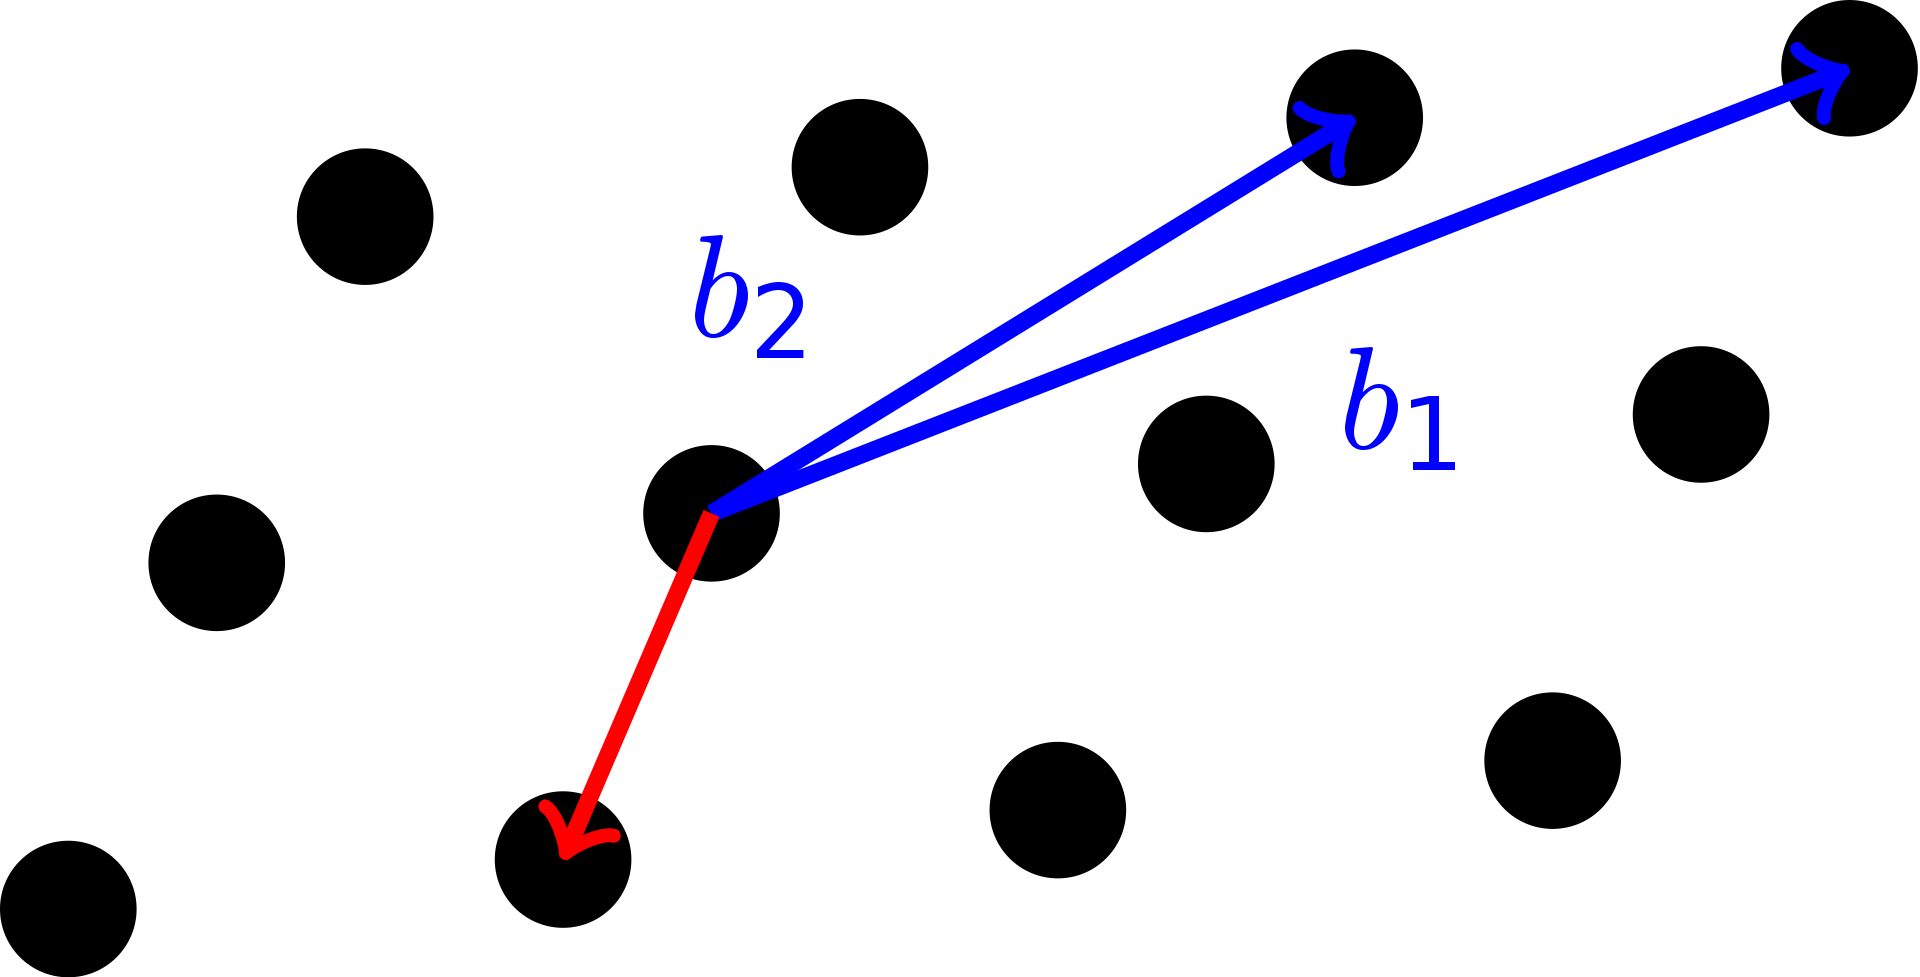
\includegraphics[scale=0.08]{problem55_1.png}
\end{figure}
To simplify this problem, just change it to finding the shortest distance from original to any non-original lattice points in that vector space. Another simplification to make is to assume that the dimension of the given basis is the same to the dimension of the vector space(which means $B$ is square). However, the hardness of the original problem is still $\mathcal{NP}$-hard

In many cases the problem can be further simplefied to be $\gamma$-approximation SVP, denoted as $SVP_{\gamma}$. This approximated problem intends to find a vector in the lattice whose length is at most $\gamma\lambda$, where $\gamma$ is a specified number larger than 1 and $\lambda$ is the theoretical shortest length. This simplication make the requirement of the optimization to be looser and in that case, there is a polynomial-time algorithm called  Lenstra-Lenstra-Lov\'asz(LLL) Algorithm, which is designed for $\gamma = 2^{(n-1)/2}$

The first step is to orthogonalize the basis. Orthogonalization of a basis $B$ is to build another basis $B^*$ which spans the same space(but possibly not same lattice) with $B$, and the vectors in $B^*$ are all orthogonal(perpendicular) to each other. Here the Gram-Schimidt algorithm (whose introduction is offered in reference) will be used for orthogonalization.

Next is to create a coefficient matrix $\mu$, in which $\mu_{i,j}$ means the weight of $b_j^*$ in the vector $b_i$ ($1\leq j<i\leq n$)

The following step is to adjust the original basis $B$ using column opeartion to make the $B^*$ and $\mu$ to maintain the LLL-Condition:

\begin{itemize}
    \item For $1\leq j<i\leq n$, $|\mu_{i,j}|\leq 0.5$
    \item Specify a real number $\delta\in(0.25,1)$ (usually $0.75$), then for $k=2,...,n,\delta \|b_{k-1}^*\|^2 \leq \|b_k^*\|^2+\mu_{k,k-1}^2\|b_{k-1}^*\|^2$
\end{itemize}

The first condition can be satisfied by subtracting $|\mu_{i,j}|b_j$ from $b_i$, and the second condition can be satisfied by just swapping columns. After the LLL-conditions are satisfied for all columns, the first column is just the vector we want to find. The mathematical proof can be found in the first reference url.

% add comment in the pseudocode: \cmt{comment}
% define a function name: \SetKwFunction{shortname}{Name of the function}
% use the defined function: \shortname{$variables$}
% use the keyword ``function'': \Fn{function name}, e.g. \Fn{\shortname{$var$}}
\begin{Algorithm}[Lenstra-Lenstra-Lov\'asz Algorithm\label{problem55}][H]
	% - replace nb with problem number (e.g. problem101)
	% -	must match the reference in the overview
	% - when writing more than one algo use problem101a, problem101b, problem101c etc.
	
	\Input{A basis $B$ of dimension $n$, a norm $\|v\|$}
    \Output{A vector in the lattice whose length is at most $2^{(n-1)/2}\lambda$}
    ortho $\leftarrow $GramSchimidt($B)=\{b_1^*,b_2^*,...b_n^*\}$\;
    k $\leftarrow 1$\;
    $\delta \leftarrow 0.75$\;
    \For {$j\leftarrow 1 \text{ to } n-1$}{
        \For {$j\leftarrow j+1 \text{ to } n$} {
            $\mu_{i,j} \leftarrow \frac{<b_i,b_j^*>}{<b_j^*,b_j^*>}$\;
        }
    }
   \While {$k<n$}{
        \For {$j\leftarrow n-1 \text{ downto }1$}{
            \uIf{$|\mu_{k,j}|>0.5$}{
                $b_k \leftarrow b_k-|\mu_{k,j}|b_j|$\;
                ortho $\leftarrow $GramSchimidt($B)=\{b_1^*,b_2^*,...b_n^*\}$\;
                \For {$j\leftarrow 1 \text{ to } n-1$}{
                    \For {$j\leftarrow j+1 \text{ to } n$} {
                        $\mu_{i,j} \leftarrow \frac{<b_i,b_j^*>}{<b_j^*,b_j^*>}$\;
                    }
                }
            }
        }
        \uIf{$\|b_k^*\|\geq (\delta-\mu_{k,k-1}^2)\|d_{k-1}^*\|$}{
            $k\leftarrow k+1$\;
        }
        \Else{
            Swap $b_k$ and $b_{k-1}$\;
            ortho $\leftarrow $GramSchimidt($B)=\{b_1^*,b_2^*,...b_n^*\}$\;
            \For {$j\leftarrow 1 \text{ to } n-1$}{
                \For {$j\leftarrow j+1 \text{ to } n$} {
                    $\mu_{i,j} \leftarrow \frac{<b_i,b_j^*>}{<b_j^*,b_j^*>}$\;
                }
            }
            $k\leftarrow max(k-1,1)$\;
        }
   }
   \Ret $b_1$
\end{Algorithm}



\subsection*{References}
% list references where to find information on the given problem
% prefer books, research articles, or internet sources that are likely to remain available over time
% as much as possible offer several options, including at least one which provide a detailed study of the problem
% if available include links to programs/code solving the problem

\begin{itemize}\itemsep .125cm
	\item \url{https://web.eecs.umich.edu/~cpeikert/lic13/lec02.pdf}
	\item \url{https://en.wikipedia.org/wiki/Lattice_problem}
	\item \url{https://www.math.hmc.edu/calculus/tutorials/gramschmidt/gramschmidt.pdf}
	\item Lenstra, A. K.; Lenstra, H. W., Jr.; Lovász, L. (1982). "Factoring polynomials with rational coefficients".
\end{itemize}

\ifx\onefile\undefined
	\end{document}
\fi
